\documentclass[12pt,oneside, a4paper]{article}
\renewcommand{\baselinestretch}{1.0} 
\usepackage[a4paper,left=1.5cm,right=1.5cm,top=1.5cm,bottom=1.5cm]{geometry}
\usepackage[brazilian]{babel}
\usepackage[utf8]{inputenc}
\usepackage[T1]{fontenc} %ACENTOS%
\usepackage{mathtools}
\usepackage{indentfirst} %Identa o paragrafo 1%
\usepackage{pslatex} %Fonte Times New Roman%
\usepackage{natbib} %Ref Bibliografica BibTEx %
\usepackage[table,xcdraw]{xcolor}%Para a tabela %
\usepackage{titlesec}
\usepackage{graphicx}

\graphicspath{{figures/}}

\begin{document}

\title{\normalfont\fontsize{14}{15}\bfseries Uma abordagem MSPL para Sistemas Múltiplos de VANT}
\author{\normalfont\fontsize{12}{15}\bfseries \textit{Junier Amorim e Ruyther Costa}}
\date{}

\maketitle

\titleformat{\section}
  {\normalfont\fontsize{12}{15}\bfseries}{\thesection}{1em}{}
\titleformat{\subsection}
  {\normalfont\fontsize{12}{15}\bfseries}{\thesubsection}{1em}{}
 
  
\section{Introdução}

O artigo que descreve uma proposta de aplicação de \textit{Swarm Intelligence (SI)} para o controle de atribuição de tarefas em um sistema múltiplo de veículos aéreos não tripulados (VANT) \cite{01}. O referido material define o conjunto de tarefas como a missão a ser cumprida pelo conjunto de VANTs, aqui também denominados de drones, e que são dotados de 1 ou mais tipos de sensores e capacidade de bateria (autonomia de vôo). Tal conjunto caracteriza o time, podendo ter mais de um time de drones. A atribuição da tarefa para o drone é de ${n:1}$, ou seja, um drone pode executar várias tarefas , e cada uma dessas, por sua vez, só podem ser cumpridas por apenas 1 drone.

A decisão de cada drone em assumir uma determinada tarefa é tomada por ele, baseado em informações locais tais como, autonomia de vôo e características dos sensores a bordo, além disso, usa-se o resultado de cálculos que atribuem peso à execução das tarefas, tal como a tendência ($\Theta$). Com isso, o comportamento do time de drones reúne uma inteligência artifical coletiva, baseada em decisões e informações locais. \cite{03}

O envio das tarefas bem como a comunicação dos drones com o centro e com outros drones é feito por intermédio de \textit{tokens}. Essa comunicação é feita em modo broadcast e por meio dela os drones ''entendem'' a situação dos demais do time.

A receber o token com as tarefas, os drones realizam o cálculo da tendência, da qualidade dos sensores embarcados ($Q_{ij}$), e da capacidade ($k_{ij}$) de execução e, se tiverem condições, escolhem a tarefa que melhor será realizada por ele, baseado nas informações locais que ele possui.

Tal problema materializa o cenário de formação de times a partir de agentes autônomos/semiautônomos \cite{04} voltas a execução de uma ou várias tarefas que compõem a missão. 

Extrapolaremos essa visão de times de agentes para Linhas de Multi Produtos de Software (Multi Software Product Lines - MSPL) onde cada agente, possuidor de uma configuração válida, caracteriza uma Linha de Produto de Software (Software Product Line - SPL) dentro da MPL. Tais SPLs representadas por Features Models (FM) contribuiriam entre sim geranto o resultado do time. Cada configuração válidade de uma SPL de modo combinado gera a variabilidade da MPL e, em consequência, do time.



\section{Fundamentação Teórica}
A modelagem do problema será realizada através do uso de SPL e MSPL representando cada um dos drones e o time, respectivamente. Nessa visão tentaremos atribuir ao sistema a capacidade de adequar-se dinamicamente a mudanças no cenário e/ou nas tarefas que serão executadas.


\subsection{Múltiplas Linhas de Produtos de Software}

Uma SPL representa programas, bibliotecas, sistemas ou componentes de software. Para um produto de elevada complexidade e heterogeneidade, a SPL se tornaria muito extensa e ramificada, inviabilizando a sua representação e ou obtenção de todos os resultados da variabilidade. Nesses casos, a estratégia é dividir em diversas SPLs autônomas que comporão a MSPL (\textit{Multi Software Product Line}) e que geram um produto final com maior complexidade.

Na MSPL temos relações entre as SPL que a compõem. Podemos definir essas relações como sendo uma dependência entre as SPLs, e que representam uma relação entre o estado atual e a reconfiguração necessária entre linhas de produtos de software. Uma configuração válida de uma SPL pode afetar a configuração de várias outras SPLs que compõem a MSPL\cite{05}.

O conjunto de todas as configurações válidas de todas as SPL definem a variabilidade da MSPL. Uma configuração válida da MSPL reúne um conjunto formado por uma configuração válida de cada uma das SPLs.

A representação de uma MSPL deve conter informações sobre as dependências funcionais mútuas entre as SPLs que a compõe, bem como as consequências de uma configuração válida de uma dada SPL sobre as demais e sobre o produto final da MSPL. Com isso, devemos ter as informações necessárias para ajustar a MSPL dado que uma SPL foi reconfigurada.

\begin{figure}[!htb]
\centering
\fbox{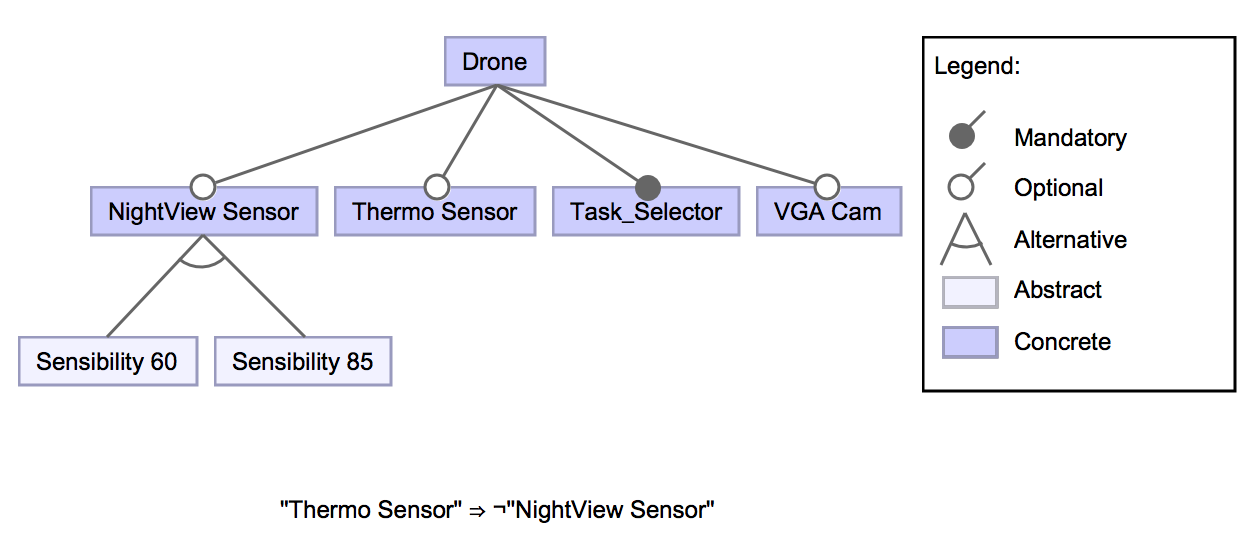
\includegraphics[scale=0.6]{fm01.png}}
\caption{Um Modelo de Feature representando um dos drones do time}
\label{figure 01}
\end{figure}

Em vez de usarmos o Modelo de Features (FM), utilizado para modelar uma SPL,  no caso da MSPL utilizaremos uma notação muito próxima à definida na Modelagem Orientada a Objetos com UML (Unified Modeling Language), proposto em \cite[Rosenmüller, 2018]{02} e denominados de Modelos de Composição.


\section{Modelagem}

A primeira modelagem necessária para o problema apresentado pelo artigo de referência \cite{01} é a dos drones que compõem o cenário. Cada drone será uma SPL que caracterízará as configurações possíveis de todos os recursos embarcados na aeronave. A representação da SPL será por meio do Modelo de Features (FM) e a Figura 01 mostra as features de uma determinada aeronave do time.

\begin{figure}[!htb]
\centering
\fbox{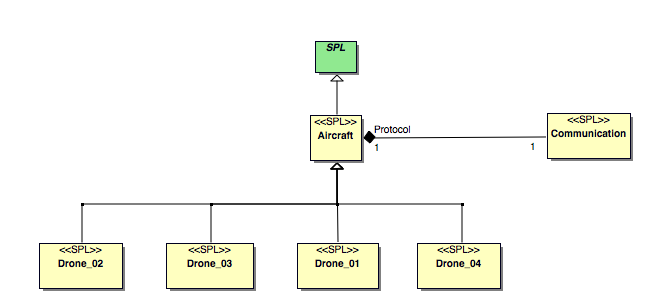
\includegraphics[scale=0.7]{uml01.png}}
\caption{Modelo de Composição da MSPL representando um time de drones}
\label{figure 02}
\end{figure}

No modelo apresentado poderemos ter restrições (constraints) aplicadas a uma ou mais features. Apesar do cenário original basear-se em \textit{Swarm-GAP}, em que a decisão de associação de problemas ser baseada exclusivamente em informações locais, na modelagem sob o aspecto de Linha de Produtos de Software expandiremos para a existência de uma comunicação broadcast entre todas as SPLs (consciência conjunta).

Com as SPLs representadas por FM, pode-se criar o Modelo de Composição, representando uma MSPL através das interações e dependências das SPL que o compõe, ocultando os detalhes de cada uma delas.

\begin{figure}[!htb]
\centering
\fbox{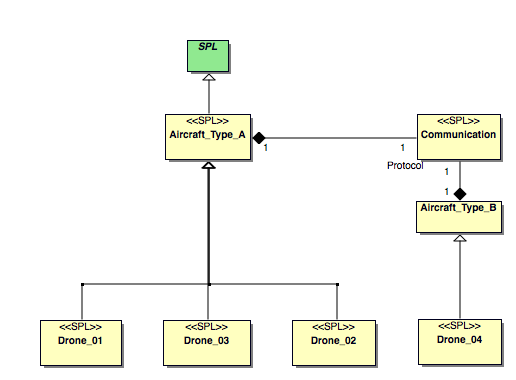
\includegraphics[scale=0.8]{uml02.png}}
\caption{Modelo de Composição da MSPL com mais especializações entre as SPL}
\label{figure 03}
\end{figure}

O Modelo de Composição pode ser criado a qualquer momento, especialmente quando houver mudanças nas SPLs que venham a alterar alguma relação entre elas ou que possa surgir novas relações entre as mesmas. Na figura 03 podemos observar que houve a adição (especialização) do tipo de aeronave baseado em alguma característica ou recurso das mesmas definidos pelas regras do Domínio/Contexto.

Nesse modelo, cada produto é uma instância (variabilidade) da linha de produtos que permite a conexão entre uma ou mais SPL. Vamos considerar a seguinte definição para o modelo de features $ FM $:

\begin{equation}
FM = (F,P)
\end{equation}


Onde $ FM $ representa um conjunto de features $ f $, e $ P $ é um conjunto de produtos válidos $ p $. Baseado nisso, podemos definir uma SPL como sendo uma relação entre o modelo de features da linha de produtos de sofwtare e o gerador $ G $ dos produtos:

\begin{equation}
SPL = (M, G)
\end{equation}

Se tivermos uma alteração no diagrama de features de uma determinada SPL, teremos um modelo de features derivado $ FM' $. Tal modelo gerará novos produtos e consequências à MSPL.

\begin{equation}
FM' = (F', P')
\end{equation}

Em uma MPL, representaremos as SPL por uma tripla: $(M, G, D)$, onde $(M,G)$ representam a SPL em si, e $D$ representa um conjunto de dependências $d_{i}$ de outras SPL que compõem a MPL. Com isso, uma dada MPL válida será representada pelo conjunto:

\begin{center}
$S=\{(M_{i},G_{i},D_{i})\}$
\end{center}

Para obtermos uma MPL válida, aplicamos um conjunto de funções a cada uma das FM das SPL componentes a fim de gerar produtos compatíveis. 

\begin{center}
$  G_{i} = \{g_{n}()\} $
\end{center}




**** TO DO *****


CSP (Constraint Satisfaction Problems) é uma estratégia de elevado custo computacional. Não é adequada para uso em equipamentos compactos e com pouco recurso de Hardware. Pode ser usada em processamento centralizado (dando uma primeira configuração válida) no caso da exstência de uma gerenciamento central.

Uso de MOEA para maximizar a confiabilidade de um FM baseado em objetivos e constraints. Algoritmo PAES (MOEA) para otimização aplicado a função de capacidade dos drones ($k_{ij}$)

O uso do algoritmo de Pareto permite levantar um conjunto de soluções possíveis (objetivos), permitindo rápida flexibilização no caso de alterações no time(conjunto de drones no caso do problema avaliado) ou no caso de atribuir mais de um alvo (task, tarefa) para cada drone.


Impactos dos resultados MOEA na formação do time de drones para o comprimento da missão (considerando a missão um conjunto de tarefas). O PAES aplicado para maximizar a confiabilidade do FM para um dado conjunto de restriçÕes (constraints)

\subsection{DSPL}

\section{XXXX}

\section{Conclusion}
....

\renewcommand{\bibfont}{\small}
\renewcommand{\baselinestretch}{1.0} 
\bibliography{ref}
\bibliographystyle{plain}

\end{document}